%!TEX program = xelatex
\documentclass[twoside,color=blue,mathpazo,titlestyle=hang,12pt]{elegantbook}
% \email{elegantlatex2e@gmail.com}
% \title{统计观点下的测量平差}
% \zhtitle{统计观点下的测量平差}
% \zhend{}
% \entitle{\ }
% \enend{}
% \version{2.10}
% \myquote{Victory won\rq t come to us unless we go to it.}
% \logo{logo.pdf}
% \cover{cover.pdf}

% title 
\setcounter{tocdepth}{2}
\numberwithin{equation}{section}


\title{\Huge\textbf{测量全生命周期支持系统}\Huge\\设 \\ 计 \\ 开 \\ 发 \\ 报 \\ 告} 
\author
{
\Large\textbf{同济大学测绘与地理信息学院} \\
1551126 余周炜 \\
1551140 王雪辰 \\
1551128 江子宇
}
\date{}

%green color
%    \definecolor{main1}{RGB}{0,120,2}
%    \definecolor{seco1}{RGB}{230,90,7}
%    \definecolor{thid1}{RGB}{0,160,152}

   \definecolor{main1}{RGB}{0,0,0}
   \definecolor{seco1}{RGB}{0,0,0}
   \definecolor{thid1}{RGB}{0,0,0}
%cyan color
   \definecolor{main2}{RGB}{0,175,152}
   \definecolor{seco2}{RGB}{239,126,30}
   \definecolor{thid2}{RGB}{120,8,13}
%blue color
   \definecolor{main3}{RGB}{100,149,237}
   \definecolor{seco3}{RGB}{180,50,131}
   \definecolor{thid3}{RGB}{7,127,128}

\usepackage{siunitx}
\usepackage[section]{placeins}
\usepackage{makecell}
\usepackage{listings}

\newcommand\mgape[1]{\gape{$\vcenter{\hbox{#1}}$}}

\newfontfamily\conso{Inconsolata}
\definecolor{mygreen}{rgb}{0,0.6,0}
\definecolor{mygray}{rgb}{0.5,0.5,0.5}
\definecolor{mymauve}{rgb}{0.58,0,0.82}
\lstset{backgroundcolor=\color{white},
% numbers=left,
numberstyle=\small,
frame=lines,
basicstyle=\conso,
columns=fullflexible,
breaklines=true,                 % automatic line breaking only at whitespace
tabsize=4,
keywordstyle=\color{blue},
commentstyle=\color{mygreen},
stringstyle=\color{mymauve}\ttfamily,
language=[Sharp]C}
% \usepackage[numbered,autolinebreaks,useliterate]{mcode}

% \usepackage{mdwlist}
\usepackage{lipsum}
\usepackage{colortbl}
\usepackage{texnames}
\usepackage{metalogo}
\usepackage{mflogo}
\usepackage{mathtools}
\usepackage{algorithm}
% \usepackage{algorithmicx}
\usepackage{algpseudocode}
\usepackage{longtable}
\usepackage{supertabular}
\usepackage{multirow}
\renewcommand{\algorithmicrequire}{\textbf{Input:}}  % Use Input in the format of Algorithm  
\renewcommand{\algorithmicensure}{\textbf{Output:}} % Use Output in the format of Algorithm 


\RequirePackage{cite}
\RequirePackage[square,numbers]{natbib}
\newlength{\notationgap}
\setlength{\notationgap}{1pc}

\newlength{\figwidth}
\setlength{\figwidth}{26pc}

\begin{document}
\frontmatter

\maketitle

\include{math_symbol}
\tableofcontents

\mainmatter

\chapter{项目简介}

本项目的名称是“测量全生命周期支持系统”,使用vs2010+arcEngine10.1开发,分为两个部分,一部分进行\textbf{辅助测量},是为测量辅助系统,另一部分\textbf{生成等高线}。

\section{项目背景}
测量实习中,数字平面地形图测绘部分需要用到CAD进行设站点、后视点选择以及地形图展绘;等高线测量部分需要用到ArcGIS生成等高线。 然而在实际的操作过程中,我们常常为找不到控制点和输入新的控制点而烦恼。例如校庆修路使控制点的位置和数量都发生了一定的变化,此时就需要对控制点进行大批量的更新。此外,在ArcMap中生成等高线需要经历生成TIN、TIN转栅格、生成等高线的过程,较为繁琐。

为了解决测量实习中的这些问题,开发了本系统,将测量过程中的各种操作用ArcEngine开发集成,使测量过程更加简单流畅。

\section{开发平台}

vs2010+ArcEngine10.1

\section{数据}

\paragraph{原始数据} 校园dwg图(包含控制点图层以及地物图层)

数据准备阶段将包含控制点的CAD图层转为point类型的shp文件,将包含建筑物的CAD图层转为polygon类型的shp文件。

\section{程序框架}

本项目主要有三个窗体,Form1为主窗体,如图\ref{fig:mainform}所示。
\begin{figure}[htbp]
\caption{主窗体}
\label{fig:mainform}
\centering
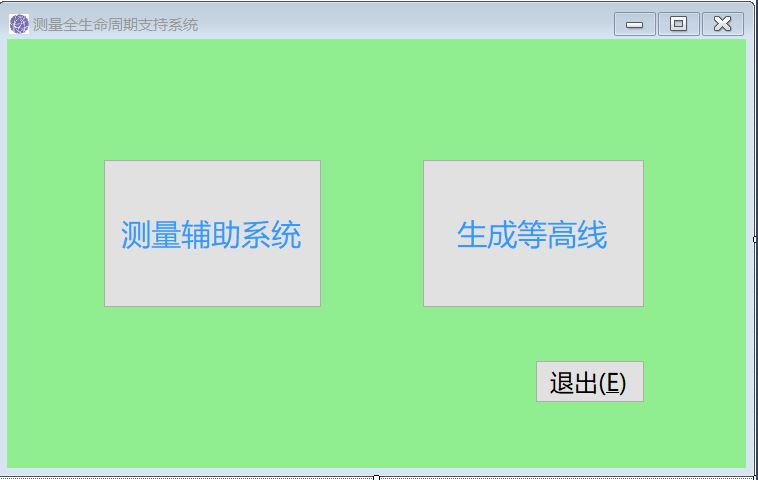
\includegraphics[width=0.8\textwidth]{mainform.JPG}
\end{figure}

第二个窗体是FormSurvey,辅助有关测量行为的进行,如图\ref{fig:forms}所示。
\begin{figure}[htbp]
\caption{FormSurvey}
\label{fig:forms}
\centering
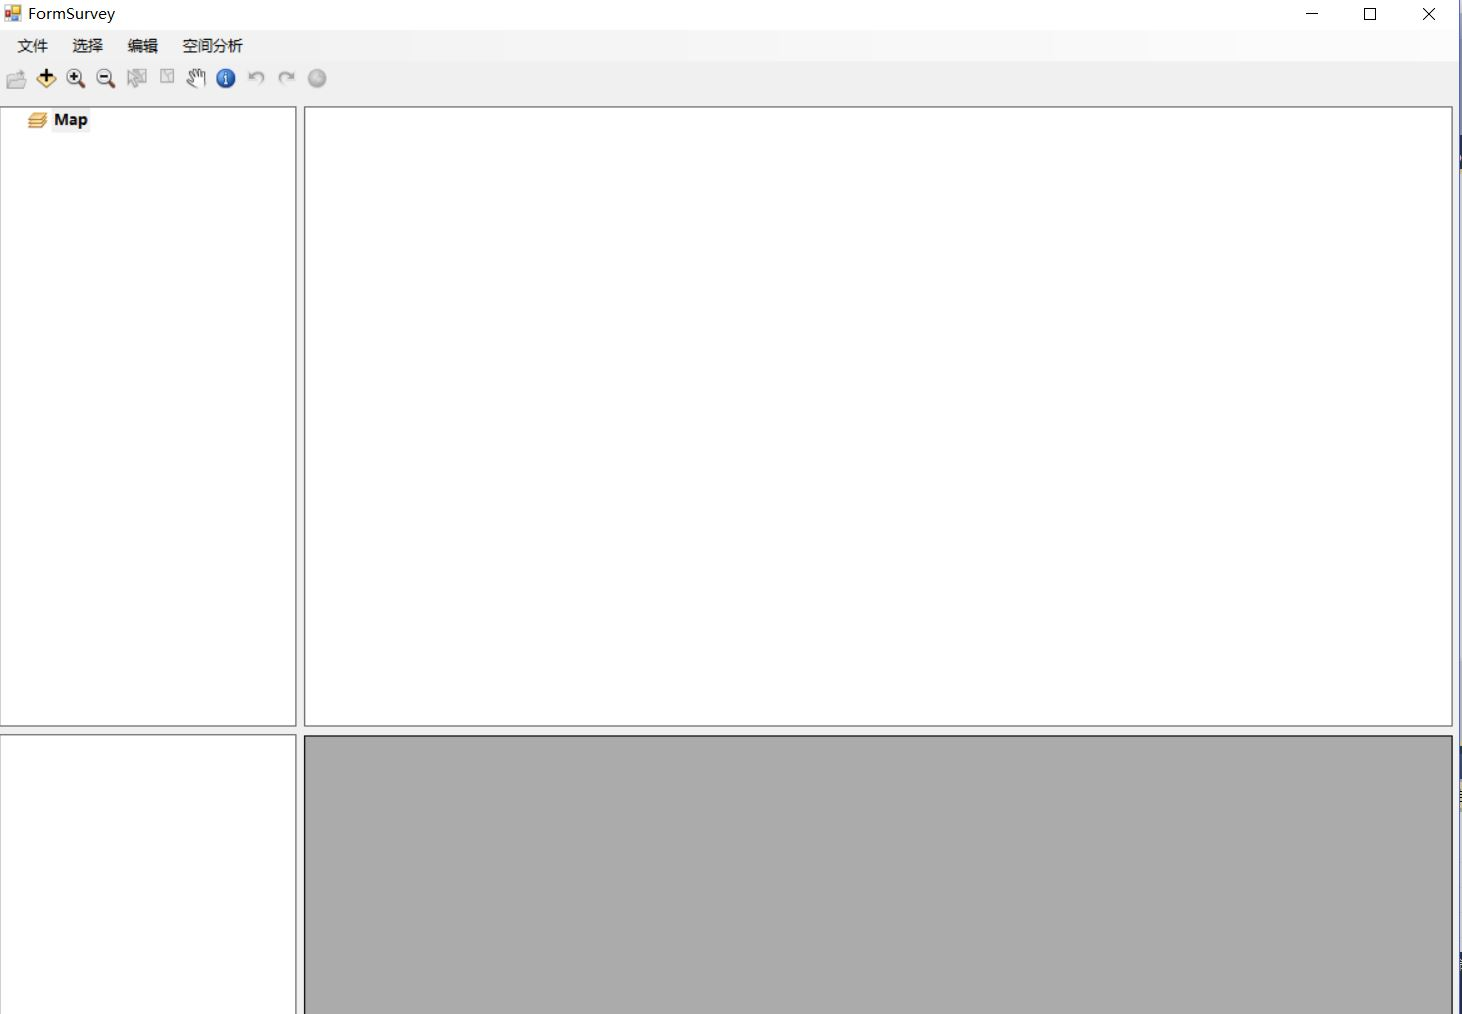
\includegraphics[width=0.8\textwidth]{forms.JPG}
\end{figure}

第三个窗体是FormCoutour,进行有关等高线的绘制,如图\ref{fig:formc}所示。
\begin{figure}[htbp]
\caption{FormCoutour}
\label{fig:formc}
\centering
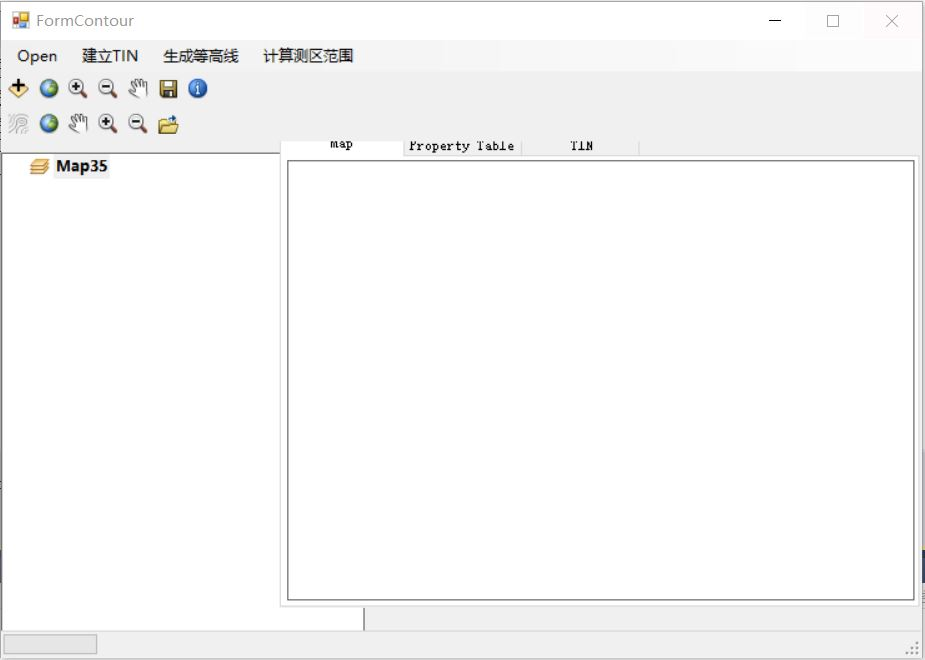
\includegraphics[width=0.8\textwidth]{formc.JPG}
\end{figure}

此外还有FormDistance,AddControlPoint等对话框。

\chapter{测量辅助系统}


\section{功能}
测量辅助系统实现了如下特色功能
\begin{enumerate}   
\item 鹰眼功能。
\item 鼠标拖动移动图层功能。
\item 输入坐标的方式添加控制点。
\item 拉框选择测区范围,显示测区边界,并将测区范围内的控制点高亮显示。
\item 选择测站所在的控制点、输入测距,在考虑遮蔽和测距的前提下给出可用的后视点。
\item 选中测站所在的控制点,给出测区范围。
\end{enumerate}

下面分别说明这些功能
\begin{description}
\item[鹰眼功能] 利用axMapControl1的OnExtentUpdated事件,当主视图范围改变时,鹰眼视图主视图在鹰眼视图中的范围同时改变。利用axMapControl2的OnMouseDown事件,当鼠标在鹰眼视图中点击时,axMapControl1的范围同时改变。
\item[图层移动] 利用axTOCControl1的OnMouseDown事件和它的HitTest方法,记录将要移动的图层,利用OnMouseUp事件和IMap的MoveLayer方法,将其移到所属的位置。
\item[选择测区范围] 单击该选项时,将bool变量flagSelectFeature置为Checked,利用axMapControl1的OnMouseDown事件和TrackRectangle()方法,记录该选框的四个角点坐标,创建一条Polyline加入axMapControl1的图形容器中。
\item[坐标添加控制点] 单击该选项时,将弹出对话框以输入坐标,单击确定时,将该坐标保存在类GlobalData的公有静态变量中,找到点图层并添加。
\item[给出后视点] 1.点击输入仪器测量选项输入仪器测程;2.以该测程为半径生成一个缓冲区;3.选取该缓冲区内的控制点和建筑物;4.对每个除测站所在控制点之外的控制点和测站点生成一条polyline,与每个建筑物求交,若该polyline与所有建筑都不相交,则选择该控制点为后视点。
\item[给出可测范围] 选中测站所在控制点,以测程为半径并显示。
\end{description}

此外,单击图层时,可以将属性表显示在下方的dataGridView中,在TOCControl中右键单击,会弹出menuStrip,将图层上移/下移或删除。还可以在选项中添加控制点,删除控制点和(随机)修改控制点符号。

\section{函数说明}

在文件FormSurvey中:
\begin{lstlisting}
public DataTable GetLayerData(IFeatureLayer layer)
\end{lstlisting}
\begin{description}
\item[作用] 从IFeatureLayer中获取属性表,并返回DataTable。
\item[描述] 利用到要素层中的要素类的Fields的FieldCount字段和get\_Field(int index)方法,得到要素类的属性表的所有字段,利用字段的AliasName作为DataTable的字段名,对于每个要素,用get\_Value(int index)方法获取其第index个字段的值。
\item[注意] 使用完FeatureCursor后要释放指针
\end{description}
\begin{lstlisting}
private void 加载Shp文件ToolStripMenuItem_Click(object sender, EventArgs e)
\end{lstlisting}
\begin{description}
\item[作用] 打开文件。
\item[描述] 运用AxMapConntrol的AddShapFile方法,添加文件。
\end{description}
\begin{lstlisting}
private void axMapControl1_OnExtentUpdated(object sender, IMapControlEvents2_OnExtentUpdatedEvent e)
\end{lstlisting}
\begin{description}
\item[作用] 更新axMapControl2的显示范围,画出axMapControl1的显示的边框。
\item[描述] 将事件的e.newEnvelope强制转换为IEnvelope,利用graphicsContainer的AddElement添加元素画出边框。注意LineSymbol,FillSymbol和RgbColor的建立。
\end{description}
\begin{lstlisting}
private void 删除图层ToolStripMenuItem_Click(object sender, EventArgs e)
\end{lstlisting}
\begin{description}
\item[作用] 删除所选图层。
\item[描述] 利用TOCControl的GetSelectedItem方法获取选中的TOCControlItem,在MapControl里找到对应图层,用MapControl的DeleteLayer方法删除该图层。
\end{description}
\begin{lstlisting}
private void axTOCControl1_OnMouseDown(object sender, ITOCControlEvents_OnMouseDownEvent e)
\end{lstlisting}
\begin{description}
\item[作用] TOCControl按下鼠标触发事件
\item[描述] 利用TOCControl的HitTest方法,获取鼠标点击的item,根据鼠标按键的不同执行不同的操作:左键将pMoveLayer置为所点击的图层,为拖动图层做铺垫,另外dataGridView显示其属性;右键弹出内容菜单。
\end{description}
\begin{lstlisting}
private void axTOCControl1_OnMouseUp(object sender, ITOCControlEvents_OnMouseUpEvent e)
\end{lstlisting}
\begin{description}
\item[作用] TOCControl抬起鼠标触发事件
\item[描述] 利用TOCControl的HitTest方法,获取鼠标点击的item,根据鼠标按键的不同执行不同的操作:左键将pMoveLayer置为所点击的图层,为拖动图层做铺垫,另外dataGridView显示其属性;右键弹出内容菜单。
\end{description}
\begin{lstlisting}
private void 选择测区范围ToolStripMenuItem_Click(object sender, EventArgs e)
\end{lstlisting}
\begin{description}
\item[作用] flagSelectFeature置为ToolStripMenuItem的Checked属性值,为axMapControl的OnMouseDown事件作铺垫。
\end{description}

\begin{lstlisting}
private void axMapControl1_OnMouseDown(object sender, IMapControlEvents2_OnMouseDownEvent e)
\end{lstlisting}
\begin{description}
\item[作用] MapControl的按下鼠标触发该事件
\item[描述] 如果flagSelectFeature为真,则调用axMapControl1的TrackRectangle方法,返回一个geometry,并利用这四个角点新建一个Polyline,并用GraphicsContainer的AddElement方法加入Polyline元素,即为测区范围;其次,创建一个spatialFilter,表示与Polygon相交,利用点图层的FeatureClass的Search方法,返回在矩形内的控制点,并将其选中高亮显示。如果flagCreateFeature为真,则创建控制点。如果flagSelectStation为真,则调用axMapControl1的TrackCircle方法,选中测站点并高亮显示。
\end{description}
\begin{lstlisting}
private void 图层上移ToolStripMenuItem_Click(object sender, EventArgs e)
\end{lstlisting}
\begin{description}
\item[作用] 将选中的图层上移一层
\item[描述] 利用axTOCControl1的GetSelectedItem方法找出选中图层,遍历所有图层,找到该图层的index,并用axMapControl1的MoveLayerTo方法将该图层上移一层。
\end{description}
\begin{lstlisting}
private void 图层下移ToolStripMenuItem_Click(object sender, EventArgs e)
\end{lstlisting}
\begin{description}
\item[作用] 将选中的图层下移一层
\item[描述] 利用axTOCControl1的GetSelectedItem方法找出选中图层,遍历所有图层,找到该图层的index,并用axMapControl1的MoveLayerTo方法将该图层下移一层。
\end{description}
\begin{lstlisting}
private void 添加控制点ToolStripMenuItem_Click(object sender, EventArgs e)
\end{lstlisting}
\begin{description}
\item[作用] 将flagCreateFeature置为添加控制点ToolStripMenuItem的Checked属性。
\end{description}
\begin{lstlisting}
private void 更换控制点符号ToolStripMenuItem_Click(object sender, EventArgs e)
\end{lstlisting}
\begin{description}
\item[作用] 更换控制点的符号
\item[描述] 选择控制点所在的图层,利用随机数,生成不同的颜色和形状,利用ISimpleMarkerSymbol 和 SimpleRenderer 设置符号和图层的渲染。
\end{description}
\begin{lstlisting}
private void 删除控制点ToolStripMenuItem_Click(object sender, EventArgs e)
\end{lstlisting}
\begin{description}
\item[作用] 将选中的控制点删除
\item[描述] 通过ISeletion和IEnumFeature接口将选中的实体遍历并用IFeature的Delete方法删除。
\end{description}
\begin{lstlisting}
private void axMapControl2_OnMouseDown(object sender, IMapControlEvents2_OnMouseDownEvent e)
\end{lstlisting}
\begin{description}
\item[作用] 在axMapControl1的地图的中心移到axMapControl2中所点的位置。
\item[描述] 利用axMapControl1的CenterAt方法即可
\end{description}
\begin{lstlisting}
private void 坐标添加控制点ToolStripMenuItem_Click(object sender, EventArgs e)
\end{lstlisting}
\begin{description}
\item[作用] 利用弹出对话框的方式,输入坐标添加控制点
\item[描述] 首先找到点图层,利用IPoint的PutCoords方法生成点,利用FeatureClass的CreateFeature()方法创建点。
\end{description}
\begin{lstlisting}
private void 选择当前测站ToolStripMenuItem_Click(object sender, EventArgs e)
\end{lstlisting}
\begin{description}
\item[作用] 将flagSelectStation置为true。
\end{description}
\begin{lstlisting}
private void dToolStripMenuItem_Click(object sender, EventArgs e)
\end{lstlisting}
\begin{description}
\item[作用] 在考虑建筑物遮挡的情况下给出可以看到的后视点。
\item[描述] 首先,建立一个半径为测程的buffer,第二,得出在buffer内的控制点和建筑物图层,第三,对每个在buffer内的非测站点,与测站点连一条线,此即为视线,判断该视线是否与建筑物相交(ITopologicalOperator的Intersect方法),如果与所有建筑物均不相交,则将其高亮显示。
\end{description}
\begin{lstlisting}
private void 输入仪器ToolStripMenuItem_Click(object sender, EventArgs e)
\end{lstlisting}
\begin{description}
\item[作用] 弹出输入仪器测程对话框。
\end{description}
\begin{lstlisting}
private void 给出可测区域ToolStripMenuItem_Click(object sender, EventArgs e)
\end{lstlisting}
\begin{description}
\item[作用] 给出可测区域的范围
\item[描述] 先以测程为半径创建一个缓冲区,然后将该缓冲区与测区范围作减运算(clip),得到可测区域范围。
\end{description}



\chapter{等高线生成系统}

等高线生成系统实现了如下特色功能
\begin{enumerate}
\item 建TIN
\item TIN转栅格
\item 生成等高线
\item 由shp文件建立TIN
\end{enumerate}

下面这对这些作详细说明。

\section{功能说明}

\subsection{读取pnt文件并保存为shp文件} 
\begin{enumerate}
\item 实现的功能\\
pnt文件是从全站仪中直接导出来的数据,是一种文本文件,每行是一条记录,记录以逗号分隔。

该步骤将pnt文件中的高程点数据读取出来,建立新的point类型的shapefile,并对其建立属性表。
\item 主要接口\\
IWorkspaceFactory,IFeatureWorkspace,IFeatureClass, IFeatureCursor,IField,IFieldEdit
\item 函数与数据组织结构
\begin{enumerate}
\item 点的数据结构
\begin{lstlisting}
struct Point3D
{
    public string ID;
    public double X;
    public double Y;
    public double Z;
}
\end{lstlisting}
\item 读取pnt文件
\begin{lstlisting}
Private List<Point3D> Read_ContourLineFile(string FileName) 
\end{lstlisting}
\item 创建shp文件对应的基本属性表
\begin{lstlisting}
private IFields CreateShapeFields(esriGeometryType p_esriGeotype)
\end{lstlisting}
\item 创建shp文件
\begin{lstlisting}
private IFeatureLayer CreateSHP_Point(List<Point3D> PointList, string FileFullPath)
\end{lstlisting}
\item 根据高程点的信息建立完整属性表
\begin{lstlisting}
private void Complete_PropertyTable(ref IFeatureClass  pFeatureClass,List<Point3D> PointList)
\end{lstlisting}
\item 显示属性表
\begin{lstlisting}
private void Display_PropertyTable(IFeatureLayer pFeatureLayer)
\end{lstlisting}
\item 打开原始测量文件
\begin{lstlisting}
private void 原始测量文件ToolStripMenuItem_Click(object sender, EventArgs e)
\end{lstlisting}
\end{enumerate}
\end{enumerate}
\subsection{建立TIN}
\begin{enumerate}
\item 实现的功能\\
由shp文件中的数据建立TIN
\item 主要的接口\\
IWorkspaceFactory ,IFeatureWorkspace,ITin,ITinEdit
\item 函数\\
\begin{enumerate}
\item TIN生成函数
\begin{lstlisting} 
private ITin Create_TIN(IFeatureClass pFeatureClass, IField pField) 
\end{lstlisting}
\item 建立TIN
\begin{lstlisting}
private void 建立TINToolStripMenuItem_Click(object sender, EventArgs e)
\end{lstlisting}
\end{enumerate}
\end{enumerate}
\subsection{生成等高线}
\begin{enumerate}
\item 实现的功能\\
根据TIN生成等高线(polyline类型的shapefile)
\item 主要接口\\
IWorkspaceFactory,IFeatureWorkspace,IFeatureClass,ITinSurface
\item 函数
\begin{enumerate}
\item 等高线生成函数
\begin{lstlisting}
private IFeatureClass Create_ContourLine(ITin pTin,string WorkSpaceName,string FileName)   
\end{lstlisting}
\item 建立TIN
\begin{lstlisting}
private void 建立TINToolStripMenuItem_Click(object sender, EventArgs e)
\end{lstlisting}
\end{enumerate}
\end{enumerate}
\subsection{测区面积量算}
\begin{enumerate}
\item 实现的功能\\
量测区域的面积(已测得的等高线覆盖的面积)。通过对高程点建立凸包,计算大约的量测面积。
\item 主要接口\\IWorkspaceFactory ,IFeatureWorkspace,IFeatureClass,
ITopologicalOperator(建立凸包),IArea(获取面积)
\item 函数
\begin{enumerate}
\item 将Point类型的pfeature转为MultiPoint,为建立凸包做准备
\begin{lstlisting}
private IFeature Convert_Point2MultiPoint(IFeatureClass PointFeatureClass)
\end{lstlisting}
\item 计算测区范围
\begin{lstlisting}
private void 计算测区范围ToolStripMenuItem_Click(object sender, EventArgs e)
\end{lstlisting}
\end{enumerate}
\end{enumerate}



\chapter{小组合作}

本小组的成员通过github进行合作及版本控制,方式是组长把程序推到github上,小组成员从组长的库中fork到自己的库中,更改后组长提出拉取请求(pull request),组长审核后将该提交合并(merge)到主分支。

Git版本控制系统中,将本地库叫master(主分支),将远程库叫origin。其他的分支这里还没有用到不讲。

\section{远程库}

github上提交的流程如图\ref{fig:cor}所示
\begin{figure}[htbp]
\caption{提交流程}
\label{fig:cor}
\centering
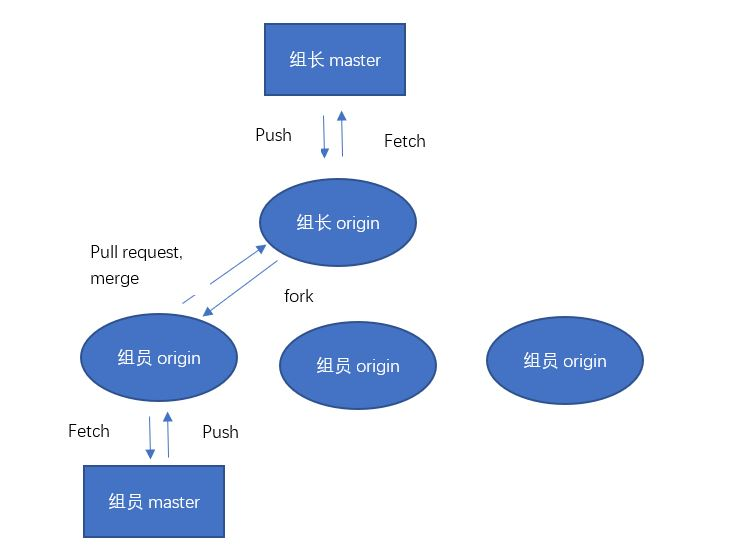
\includegraphics[width=\textwidth]{corporation.JPG}
\end{figure}

需要说明的是,因为主场的远程库在不停变动,所以组员在每次修改之前,需要先\emph{merge}组长的远程分支到master,然后才能进行修改。

\section{本地库}

下面针对本地库作讲解。在本地库中,将你选择建立git的文件夹称为工作区,add之后到暂存区,commit之后到master(主分支)。

git本地的操作如图所示\ref{fig:desktop}所示
\begin{figure}[htbp]
\caption{git本地操作}
\label{fig:desktop}
\centering
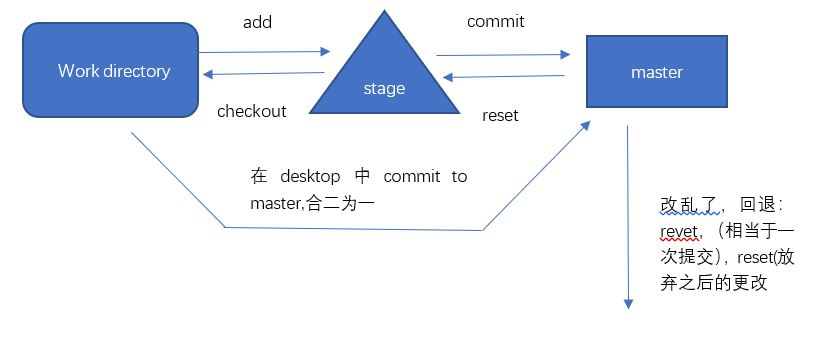
\includegraphics[width=\textwidth]{desktop.JPG}
\end{figure}

\chapter{提交文件}

\begin{table}[htbp]
\centering
\caption{文件}
\begin{tabular}{p{3cm}p{7cm}}
项目文件 & ArcEngineProgram/ArcEngineProgram.sln  \\
源代码 & ArcEngineProgram/ArcEngineProgram/*.cs \\
编译好的程序 & ArcEngineProgram/ArcEngineProgram/bin/Debug/ArcEngineProgram \\
说明文件 & document.tex,document.pdf \\
数据 & gis/pointt.shp,polygon.shp,高程数据/CL05.pnt 
\end{tabular}
\end{table}

\end{document}
